\documentclass[12pt,letterpaper]{article}
\usepackage[latin1]{inputenc}
\usepackage{amsmath}
\usepackage{amsfonts}
\usepackage{amssymb}

% the above packages are the "base"

\usepackage{graphicx}

\usepackage{hyperref} % enable links within pdf
\hypersetup{colorlinks = true, linkcolor = black, urlcolor = blue}

\usepackage{float} % for [H] forcing of figure placement

\usepackage{listings}
\lstset{basicstyle=\ttfamily,
	breaklines = true,
	tabsize=2}


\setcounter{secnumdepth}{0}  % don't number sections (stars not needed)


\author{}
\title{More with \texttt{Git} and \texttt{GitHub}}

\begin{document}
\maketitle

\tableofcontents

\pagebreak

By now you've hopefully gotten into a new routine of working with \texttt{Git} (\emph{pull, edit, commit, push}) and are doing well to remember the \texttt{Git} motto: \emph{commit early, commit often}.
Hopefully your repository is also looking nothing like Fig.~\ref{fig:makcvs}.
The goal for today is to extend our workflow by making it more flexible and adaptable to more diverse project structures and more general research contexts (such as collaborative projects).
To do that, we'll learn the basics of a few more tools that \texttt{Git} and \texttt{GitHub} offer.
Almost all of what we'll talk about below can be done using a \texttt{Git} GUI and on \texttt{GitHub}, but I might often describe actions using the command-line process.

\begin{figure}[h]
	\centering
	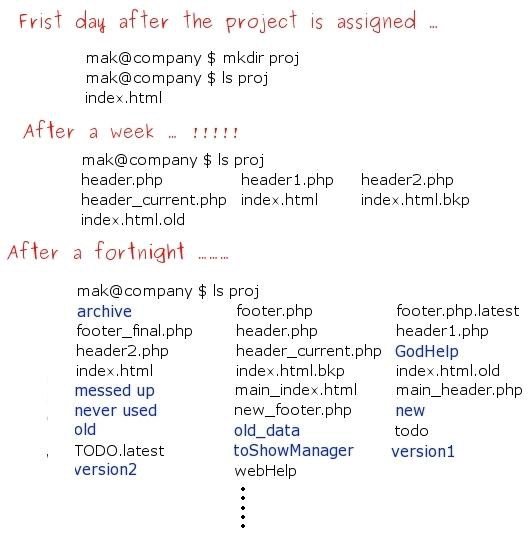
\includegraphics[width=0.8\linewidth]{figs/makcvs.png}
	\caption{The whole point of a version control system is to avoid your project folder devolving into this! (source: \url{http://maktoons.blogspot.com/2009/06/if-dont-use-version-control-system.html})}
	\label{fig:makcvs}
\end{figure}


\section{What to (\emph{not}) commit}

Up to this point, under the guiding principle of reproducibility, we've implied (if not explicitly stated) that everything associated with your project should be kept in your version control respository.\footnote{It should go without saying that anything private (e.g., passwords) should never be put in a public repository, but be careful not to do that when we start submitting jobs to High Performance Computing clusters!}
That's not entirely incorrect, but it's also not entirely true.
For example, \texttt{Git} will throw an overridable warning when you commit large files (currently $\ge 10$mb), and \texttt{GitHub} will throw a fatal error when you try to push very large files (currently $\ge 100$mb)\footnote{If necessary, you could use the Large File Storage extension: \url{https://git-lfs.github.com}}.
The latter can happen with specialized data files (e.g., GIS shapefiles).
\texttt{GitHub} also as a limit on the total size of any one repository ($???$mb).
Sometimes it's therefore necessary to keep some files in a different directory outside of your repository (preferably tracked by \texttt{Dropbox} or similar cloud storage).\footnote{See back to our \texttt{Structured Projects} class.}
Sometimes it's possible to cut-up your data into smaller pieces.
Other times, and more generally speaking, it's possible to reduce the size of a file by saving its contents in a different format, a plain-text format.

What I mean by plain-text format is most easily seen by comparing the contents of a data worksheet saved in a \texttt{.csv} file or text saved in a \texttt{.txt} file to the same data or text saved in, for example, a Microsoft Excel \texttt{.xls} or Word \texttt{.doc} file.
The former are human-readable when opened and edited in even the most basic of text editors.
In contrast, if you were to force open the \texttt{.xls} or \texttt{.doc} files in the same text editor you'd get a whole bunch of unintelligible and indecipherable computer symbols.
That's because the \texttt{.xls} and \texttt{.doc} files are binary files and have a whole bunch of additonal information in them for interpreting, presenting and otherwise doing things (e.g., calculations) with your data and text that requires specialized software.\footnote{\texttt{.Rdata} files are also binary files that need R to open them.}
We don't want all that extra stuff for a few reasons:
\begin{enumerate}
 	\item your data should contain nothing but data;
	\item we're going to do all calculations by script so as to make them reproducible and readable;
	\item your text documents should remain readable even in 10 years time and even after Microsoft Word has yet again updated to save things in a new way;
 	\item every time you open and save a \texttt{.xls} or \texttt{.doc} file, a whole bunch of that computer language information is changed, causing \texttt{Git} to unnecessarily track these changes;
	\item we want to make it easy on us to visualize exactly what content has changed in a file since it was last committed (or between any two commits) using a \texttt{Diff} tool that we'll talk about below.
\end{enumerate}
So challenge yourself to use plain-text file formats whenever possible.
Plain-text files include \texttt{.csv} files, \texttt{.R} scripts, Markdown \texttt{.md} scripts, and \LaTeX\ \texttt{.tex} files.
Images (e.g., \texttt{.jpeg}) and movies (e.g., \texttt{.mp4}) are not.\footnote{Their large file size also makes \texttt{Git} and \texttt{GitHub} a poor place to store large amounts of image and movie files.}
Microsoft- and Apple suite files and the like are (mostly) not plain-text files.

Other types of files you should not commit are temporary files, such as \texttt{\$.xls} files that are generated only when a program like Microsoft Excel is open, or anything but the primary \LaTeX\ \texttt{.tex} (and perhaps the associated \texttt{.pdf}) file (because these all get generated each time you compile your document).
You should also not commit your \texttt{.Rprofile} file (since it contains proprietary API keys).
All these temporary file types can be added to your \texttt{.gitignore} file.


\subsection{Untracking files}
What to do when you accidentally commit a file you don't want \texttt{Git} to track (e.g., you forgot to add it to \texttt{.gitignore}), or if you change your mind about a particular file and no longer want to track it?
If you're using a \texttt{Git GUI}, you can probably just right-click the file and select \texttt{Untrack} or \texttt{Stop tracking}.
To remove the file from the staging area via command-line, use \texttt{\$git rm --cached \emph{filename}}.  To remove the file entirely (i.e. from the repository), use \texttt{\$git rm \emph{filename}} (without the \texttt{--cached}).


\section{Branching}
So far, when we've committed to our \texttt{Git} repository, we've been doing so to its \emph{master} branch.
The \emph{master} branch has been our only branch, and every change we've made to a file has been changed sequentially (i.e. has overwritten what was there before).
In other words, our commit workflow has been pretty much linear.

But there are often times when you have an idea for doing something differently.
You might have an idea for optimizing a section of code (e.g., by vectorizing the use of a function, rather than using a \texttt{for} loop\footnote{See \texttt{Faster Computing} class later.}), or you might want to try writing a section or paragraph of your manuscript a different way\footnote{Or you just got rejected from \emph{journal-that-doesn't-deserve-to-publish-your-work-anyway} and want to reformat your manuscript for another journal, but want to hang on to the original because you may need to move to journal \#3 and would  want to start from the first journal's version to do so.}.
In both cases you don't want to ``break'' what's already there and working, but just want to try out an alternative.
Branches are the way to do that in \texttt{Git}.
In the \texttt{Git} supporting documents, a branch for trying something out (i.e. adding a new feature) is often referred to as the ``\emph{feature branch}.''

Creating a branch is easy.
In your \texttt{Git} GUI there's probably a button for doing so at the top of 
the interface.
You can also do it within \texttt{RStudio} and on \texttt{GitHub}.
To create a branch using command-line, type \texttt{\$git checkout -b \emph{branchname}}.
\texttt{Git} will not duplicate any of your files, but it will keep track of all changes made within the branch (when you commit them to the branch).
If you add, edit, or remove files (and commit) while your on your feature branch, those changes will not appear in your master branch (and vice versa).
Thus, if you were to add a file while in your feature branch and were then to switch back to the master branch (using your \texttt{Git} GUI, RStudio, or \texttt{\$git checkout master}\footnote{Note that the \texttt{-b} used previously was only to create the new branch; you don't use it to switch to an existing branch.}), you wouldn't see that new file your project directory.

The best way to think about your \emph{master} branch is the way a software developer would:
the master branch contains your clean, functioning, usable software (or as close as you are to developing it).
All other branches are for trying things out.
You may end up with many parallel branches, one each for testing out changes to each of several scripts or manuscript sections.
Only once you're satisfied with your changes on the feature branch, and have made sure that they work as intended for their specific purpose and in the grand scheme of things (i.e. they don't introduce bugs or affect problems elsewhere in your code), do you bring them back into the master branch and override what was there.
That's done by \emph{merging} the feature branch into the master branch (see next section).

The other context in which branches are extremely useful is in collaborative settings where you're working on analyses or a manuscript with others.
The workflow is similar to the above in that the master branch contains the not-to-be-broken best of what you've got.
Each collaborator creates task-specific branches in which to work (e.g., ``I'll work on (re)writing the Methods section,'' or ``I'll work on a script to do this part of the analysis.'')\footnote{Remember to make sure your local master branch is up-to-date before creating a branch by first doing a \emph{Pull} from \texttt{GitHub} before you create a branch.}.
Then, in collaborative contexts, it's often useful to add one more step before merging:  to issue a \emph{Pull Request} (in \texttt{GitHub}) that asks the other person to review your work before implementing the merge (see below).

Now at some point you will probably end up with more than one feature branch.
You might even have created feature branches off other feature branches.
Or you might like to go back and look at the branching relationships and history of your repository.
While \texttt{Git} has a command-line way of visualizing this history, the visualizations provided by \texttt{Git GUI}s are more informative and easier to navigate (Fig.~\ref{fig:stbranch}).
You can also use \texttt{GitHub} to see the history by going to \texttt{Insights>Network} (Fig.~\ref{fig:ghbranch}).
(It can take a while for the graph to generate.)

\begin{figure}[h]
	\centering
	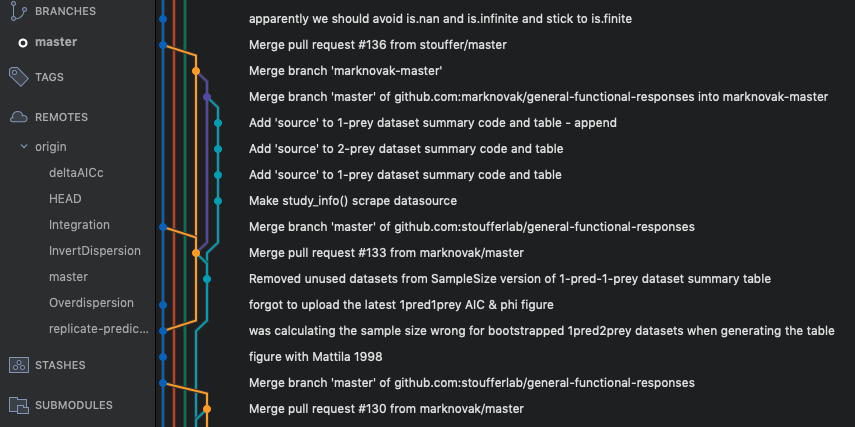
\includegraphics[width=0.8\linewidth]{figs/SourceTree_branches.png}
	\caption{\texttt{SourceTree}'s branch visualization.}
	\label{fig:stbranch}
\end{figure}

\begin{figure}[h]
	\centering
	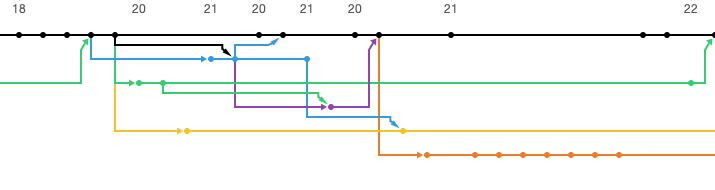
\includegraphics[width=1\linewidth]{figs/GitHub_branches.png}
	\caption{\texttt{GitHub}'s ``Network'' branch visualization.}
	\label{fig:ghbranch}
\end{figure}



\section{Differencing \& Merging}

\subsection{\texttt{diff} for highlighting changes}
So now you've made changes to your code or manuscript, but before you commit those changes you'd like to compare what you've done to what you had before (in the same branch).
That's easy using \texttt{RStudio} or any \texttt{Git GUI}.
In \texttt{RStudio} you can see the changes by clicking on \texttt{Diff} (or \texttt{Commit}) and selecting the specific file from within the staging area.
Red lines of code with minus symbols at the start are removals, green lines of code with plus symbols are additions.
In \texttt{SourceTree} and most other \texttt{Git GUI}s, simply selecting the specific file in the ``unstaged'' area will cause the changed lines to be shown in an adjacent window with similar highlighting.\footnote{When you start using \LaTeX, notice that \texttt{Git} can only differentiate lines ending in a hard-return.
Hence, any sentences or paragraphs that use line-wrapping won't be differentiated, causing even just a single-word edit to make \texttt{Git} think the whole sentence/paragraph has changed.}

Similarly, using \texttt{Git GUI}s or command-line \texttt{Git}, you can compare the changes between your current working files and an older commit, or between any pair of commits within your branch or across branches.
In \texttt{SourceTree}, simply view the \emph{History} and select the two commits you want to compare using \texttt{Ctrl + left click}.
For command-line options, see \url{https://git-scm.com/docs/git-diff}.


\subsection{\texttt{merge} for collapsing branches}

You're happy with what's in your feature branch and are ready to bring it into your master branch.
In many cases (when there are no conflicts) this is exceptionally easy.
In your \texttt{Git GUI}, simply switch to the branch (i.e. the master branch) into which you'd like to merge the feature branch, click on the \emph{merge} button, select the feature branch, merge, and commit the new changes with a useful commit message.
For command-line, use \texttt{\$git merge \emph{feature branch}} and then commit.
Remember:  If you're working collaboratively, make sure your local copy of the master branch is up-to-date by doing a \emph{Pull} from \texttt{GitHub} before attempting to merge (as you did before creating the feature branch).
That will help a lot to reduce merge conflicts\footnote{Just like being clear with your collaborator regarding what sections you're working on so that they don't work on the same sections (though this isn't a fundamental problem).}.

Now, something to consider before you merge branches is your merging pattern.
The most obvious pattern is to merge your feature branch into your master branch.
That's the quickest, and introduces little risk when you're working solo or when you're adding new files that are unlikely to entail merge conflicts.
The alternative to consider (especially in collaborative settings) is to merge the master branch into your feature branch, test that everthing works, then merge the updated feature branch back into the master.
This pattern reduces the risk of new bugs in the master that may have be introduced by having two sets of parallel changes.
It also reduces the risk of having to resolve merge conflicts on the master branch, which could affect your collaborator's ongoing efforts.
The disadvantage of this second merge pattern is that it takes an extra step and results in double the number of merge commits.
An alternative that solves this problem is \emph{rebasing}, but that comes with other potential challenges.\footnote{\url{https://git-scm.com/book/it/v2/Git-Branching-Rebasing}}

When there are no conflicts, \texttt{Git} will simply amalgamate\footnote{fanciest sounding synonym for merge I can think of} the two branches.
If you're happy with the result (which you certainly should be if you've followed the second merge pattern), then you can delete the feature branch (e.g., \texttt{\$git branch -d \emph{branchname}}).

\subsection{Resolving merge conflicts}

When \texttt{Git} notices that the same line of code has been changed on both the feature branch and the master branch subsequent to the feature branch having been created, it will tell you that there's a conflict.
Either you or your collaborator may have made the change on the master;
how should \texttt{Git} know which of these parallel changes should take precedence?
When that happens, you'll have to resolve the conflict manually, then commit those fixes before being able to proceed.\footnote{Admittedly, this \emph{can sometimes} be a little annoying until you get the hang of it.}

First, identify the file that contains the conflict.
Your \texttt{Git GUI} should have identified the problem file(s), but you can also use \texttt{\$git status} via command-line.
Open the file in your text editor and search the file for the conflict marker $<<<<<<<$.
Changes present in the HEAD (in our case master branch) will be after the line $<<<<<<<$ \texttt{HEAD}.
Next, you'll see $======$, which divides these changes from the changes in the feature branch, followed by $>>>>>>>$ \texttt{\emph{featurebranch}}.
In the example below, one person edited the focal sentence in the master branch to read ``feature branch into the master branch'', while the other person edited the same sentence in the feature branch to read ``master branch into the feature branch''.

\begin{lstlisting}[language=bash]
	I prefer to merge branches by merging the
	<<<<<<< HEAD
	feature branch into the master branch.
	=======
	master branch into the feature branch.
	>>>>>>> featurebranch
\end{lstlisting}

\noindent
Edit the sentence the way you want it to read (you can change it entirely if you'd like), remove all the lines that have $<<<<$, $>>>>$ or $====$ in them (i.e. create clean text), save the file, commit the change, and you're good to go.


\subsection{Pull Requests}

Merging branches (as we just did) can also be done in \texttt{GitHub} by creating a \emph{Pull Request}.
When you create a pull request in \texttt{GitHub}, there's a text box for (optionally) describing the changes that you're suggesting should be merged into the master branch.
Once submitted, a Pull Request initiates a process in which \texttt{GitHub} compares the two branches you selected (using \texttt{diff}) but then, regardless of whether there are conflicts, offers your collaborators (to whom you can assign the task of reviewing) the opportunity to add comments or request additional changes to your feature code before the merge is performed\footnote{Note that you can create a Pull Request and perform the merge yourself; you don't need to have a collaborator to use \texttt{GitHub} for merging.}.

Note that you can initiate a Pull Request at any point during your coding process, even if all you want to do is share screenshots or general ideas, or when you're stuck and need an additional brain to think about the problem.
Also, note that you can also continue to commit additional changes and push to the feature branch even after having initiated a Pull Request for it.
\texttt{GitHub} will show include these additional commits in the Pull Request view, so you can go back-and-forth with your collaborators, commenting and making revisions, until you're ready to merge.



\section{Forks vs. clones \& branches}

Cloning your project is what you did at the very start of this class when you created your repository on \texttt{GitHub}, copied the url link to it, and then provided that link to \texttt{RStudio}, your \texttt{Git GUI}, or \texttt{Git} itself to initiate the copying of everything that was on \texttt{GitHub} onto your hard-drive.
You could also have gone the other way:  create the \texttt{Git} repository on your hard-drive and then clone it to \texttt{GitHub}.
You can work on your project from multiple computers by cloning the repository to them.
(Just remember to commit and push what you're working on on the first computer in order to pull and keep working on it on your second computer.)
You are the owner of that repository.
Only you can pull and push to it unless you've granted permission for a collaborator to so\footnote{Go to the repository's \emph{Settings$>$Manage Access} in \texttt{GitHub}.}.
In fact, whether public or private, you and your permission-granted collaborators are the only one that can do anything to the repository (such as create branches).

Forks are in many ways similar but are different from branches, and serve a different purpose.
Anyone can fork a public repository.
When you fork someone's respository you create a copy of their repository over which you have control.
A reason for doing that might be wanting to contribute to someone else's project (e.g., a consortium of biologists all contributing to the maintenance of a database, or a team of R-package developers).
Or it might be that you want to use someone's project (or even one of your own old projects) as a starting point for your own new project.
What forking does is maintain a connection between the parent repository and the  descendent repository (as opposed to simply copying files, the way you would do without \texttt{GitHub}).
This permits the added convenience of being able to submit Pull Requests between forks, either to offer your improvements or additions to the parent repository, or to pull in added improvements or fixes to bugs that were identified subsequent to your having created the fork.
Just as for branches, you issue a Pull Request using the ``Compare and Pull Request'' button, but this time you'll compare across forks rather than your internal branches.



\section{Going back in time}

We already talked about how easy it is to use \texttt{diff} to compare back to prior commits, or to compare any two commits in your repository's history.
But what if you want to go back in time to revert to one of those previous commits?

\subsection{Undoing commit(s)}
If it's only your last commit that was made in error and you want to undo it, you have a few command-line options using \texttt{reset}\footnote{If you just want to make a small change to the last commit (e.g., you forgot to include a file or had a typo), you can \texttt{amend} the last commit without creating a new commit.
Note, however, that this is changing history(!), and cannot itself be amended.}.
To undo the last commit completely, use \texttt{git reset --hard HEAD\^}.
Changes that were made after the commit-before-last will be lost forever.
To undo the last commit but keep your subsequently-changed files in the \emph{unstaged} state, use \texttt{git reset HEAD\^}.
Changes that were made after the commit-before-last will remain but will be unstaged. To instead keep the changed files in the \emph{staged} state, use \texttt{git reset --soft HEAD\^}.
To revert to any older commit you'll need its ID number.
There are many additional options too, including the option to revert just a single file.
(See \url{https://git-scm.com/docs/git-reset} for more.)

In \texttt{SourceTree} you can do the same things by right-clicking on the commit you'd like to revert to (not necessarily the commit-before-last) and selecting \texttt{Reset master to this commit}.
For the latter you'll then be presented with three options: \emph{hard}, \emph{mixed}, or \emph{soft}.
\emph{hard} will cause all changes that were made after the selected commit to  be lost forever.
\emph{mixed} (the default) will keep all changed files in the \emph{unstaged} state.
\emph{soft} will keep all changed files in the \emph{staged} state.
If it's just the last commit you'd like to undo you can also right-click on the erronous last commit and select \texttt{Reverse commit}.
This won't delete the erronous commit (as the above options do) but rather will simply create a new commit equivalent to the commit-before-last.
Note that if there are commits pushed to \texttt{GitHub} (by a collaborator) that you didn't first pull, those commits will ``come back'' the next time you pull.

One thing to recognize when you're using \texttt{GitHub}:
Your last push to \texttt{GitHub} is your final recovery scenario in that you can always delete your entire local repository and re-clone (Fig.~\ref{fig:gitreset}).
Sometimes you end up messing things up enough to make that the easiest option.

\begin{figure}[h]
	\centering
	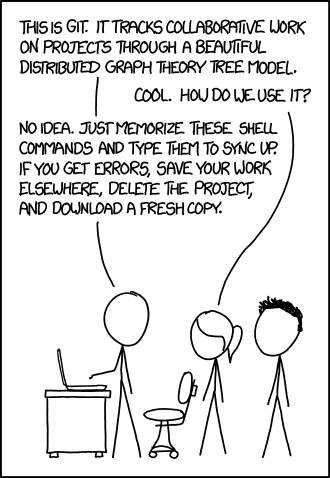
\includegraphics[width=0.5\linewidth]{figs/gitreset.png}
	\caption{Solving errors in Git (source: \url{https://xkcd.com/1597/})}
	\label{fig:gitreset}
\end{figure}



\subsection{Recapturing older commits}
You may at some point realize that you had something in a previous commit that's worth rescuing from the past. But you may not want to discard or go through the trouble of reintegrating all the subsequent work you did, as may be necessary when using \texttt{reset}.
There are a few workflows that people use to retrieve the past.
For example, to retrieve specific files or directories from an old commit, use
\texttt{git checkout \emph{commitID} \emph{filename1} \emph{dir1} \emph{dir2}} then commit, but note that this will overwrite the current copies of the files.
To retrieve and reuse a whole commit, \emph{checkout} the old commit in question, create a new \emph{branch} off the old commit, then \emph{merge} back into your master commit and resolve the conflicts in the process.
The processes are equivalent in \texttt{SourceTree} when you right-click on the old commit or files.
Notice that in the latter method lies an important reason for the \texttt{Git} motto, \emph{commit early, commit often.}
The more frequently you commit (and the better you are at commiting good ``units'' of change), the more targeted (and cleaner) your strikes to the past can be.




\section{Project Management}
Everyone has their own ways of managing their life, keeping track of To-Do's, etc.
Not surprisingly, that's true for research projects as well.
However, when you're already using \texttt{Git} to keep track of the contents of your project, its tight integration with \texttt{GitHub} enables a few very nice conveniences to keep track of both the project and its management in one place.
These features are useful not only in collaborative contexts but also when working solo.
We'll touch on only two of them, and only by means of a barebones introduction.
Other features include the ability to host project-specific websites\footnote{You can even use \texttt{GitHub} to host your own personal website.} and to create Wiki pages (which you could use as a lab notebook or to create a user manual).


\subsection{Issue tracking}
By now you've undoubtedly already seen \texttt{GitHub}'s Issue tracking interface.
The basics are pretty simple.
Create a short, specific, informative and usefully-unique subject.
Be concise and clear in your subsequent description of the issue.
You can use \texttt{Markdown} to format your comment, and use \emph{Preview} to make sure it looks right before posting.
When your issue is related to a previously-posted issue (even a closed one), link to it using \emph{$\#$issueID}.
When applicable, tag your issue with a label.
You can add to or edit the default labels to make them more useful for specific project.
By assigning issues or using \emph{@mentions} in your comment, others will receive a notifcation (or email, if they're set up to receive them in their notification preferences).
When you close an issue, it's wise to reference the commit in which the fix was enacted.
You can always reopen an issue.
To see all closed issues in the list of issues, simply delete the default contents of the filter search (i.e. delete \emph{``is:open''}).
If you've already setup a \emph{Project board}, you can also assign the issue to it.


\subsection{Project boards}
There are a number of stand-alone apps that provide so-called Kanban boards for project management.
The most basic setup entails three columns -- \emph{To do}, \emph{In Progress}, and \emph{Done}.
When you have a new task that needs doing, you add a card to the \emph{To do} column, then move it over to the next column as your actions on it progress.

In \texttt{GitHub} you can have multiple project boards per repository and use them for anything you'd use stand-alone Kanban app for.
In my mind the motivation to use \texttt{GitHub}'s project board feature is that
(1) everything to do with your project is in one place (major downside being it's only online), and that
(2) they integrate nicely with Issues.
Assigning an issue to a project board will cause it to appear in the ``To do'' column.
Closing the issue will move it to the ``Done'' column
You can set up your project board so that any newly-created issues are automatically added to the ``To do'' column.


\end{document}
